\documentclass[usenames,dvipsnames,french]{beamer}

\mode<presentation> {

\usetheme{Montpellier}
}

\usepackage{graphicx} % Allows including images
\usepackage[frenchb]{babel}
\usepackage[T1]{fontenc}
\usepackage[utf8]{inputenc}
% \usepackage[demo]{graphicx}
% \usepackage{caption}

\usepackage{subcaption}
% \usepackage{subfig}
% \usepackage{algorithm,algorithmic}
\usepackage{algorithm2e}
\usepackage{listings}
% \usepackage{ntheorem}
\usepackage{booktabs} % Allows the use of \toprule, \midrule and \bottomrule in tables
\setcounter{tocdepth}{2}
\graphicspath{{../../Figures/}}


% exercices comptés
\newcounter{numexos}%Création d'un compteur qui s'appelle numexos
\setcounter{numexos}{0}%initialisation du compteur
\newcommand{\exercice}[1]{%Création d'une macro ayant un paramètre
\addtocounter{numexos}{1}%chaque fois que cette macro est appelée, elle ajoute 1 au compteur numexos
\textcolor{DarkOrchid}{Exercice\,\thenumexos\,:}\,#1%Met en rouge Exercice et la valeur du compteur appelée par \thenumeexos
}
%----------------------------------------------------------------------------------------
%	TITLE PAGE
%----------------------------------------------------------------------------------------

\setbeamertemplate{title page}{
    \centering

    \Large\bfseries
    Machine learning Tek 5: overview of mathematical tools
    

\begin{figure}[!h]

\includegraphics[width=8cm]{fitted_distribution_1}
\end{figure}

    }

\begin{document}

\frame{\titlepage}

\begin{frame}
\tableofcontents
\end{frame}

\section{Probabilities and statistics}

\begin{frame}{}
    To have a solid understanding of machine learning, it is necessary
    to be familiar with elementary probabilities and statistics.
\end{frame}

\begin{frame}{Random variables}
\begin{figure}[htpb]
    \centering
    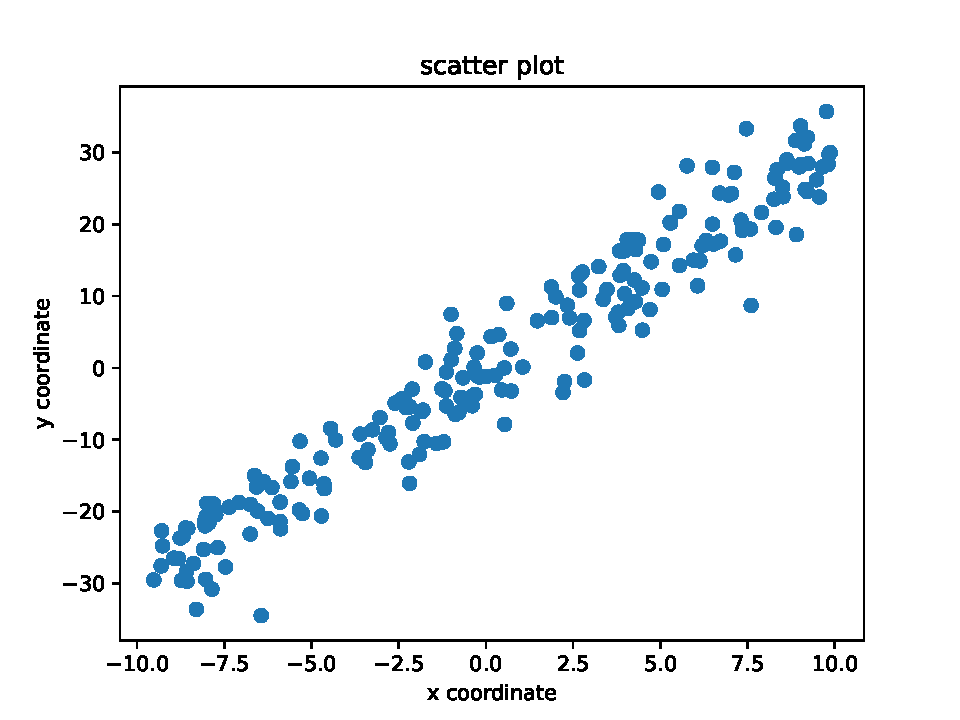
\includegraphics[width=0.8\linewidth]{simple_scatter_plot}
    \label{fig:simple_scatter_plot}
\end{figure}    
\end{frame}


\begin{frame}{Random variables}
\begin{figure}[htpb]
    \centering
    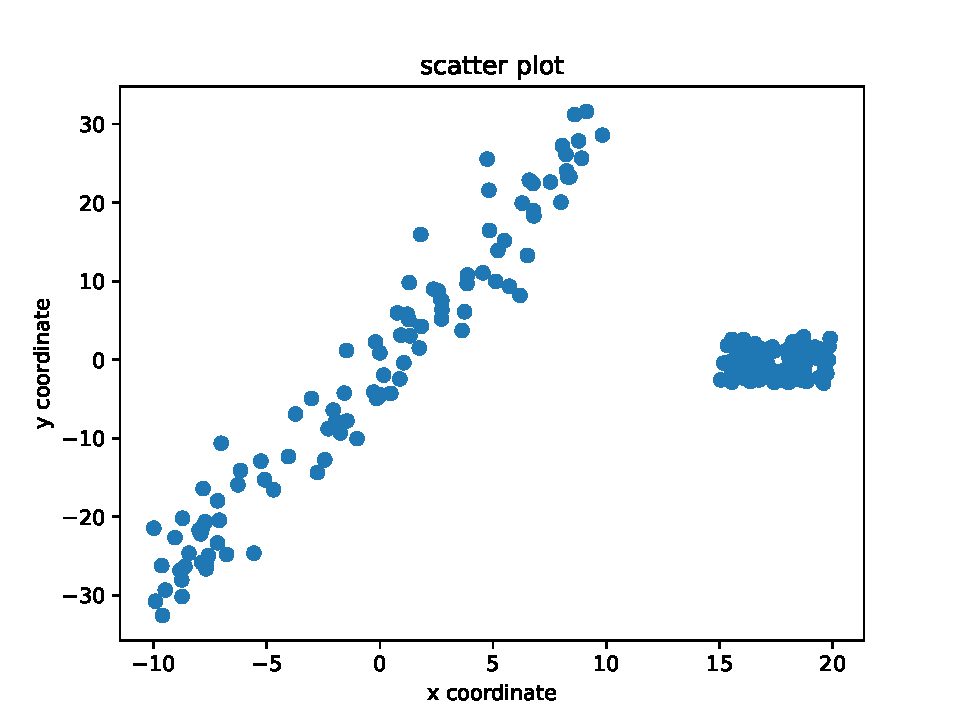
\includegraphics[width=0.6\linewidth]{different_scatter_plot}
    \label{fig:simple_scatter_plot}
\end{figure}    
We want to analyse how the data are \textbf{{distributed.}} For instance the $x$ coordinate, the $y$ coordinate.
\end{frame}


\begin{frame}
\frametitle{Random variables}
\begin{itemize}
    \item (informal definition) A \textbf{random variable} is a quantity that can take several values, with some randomness.
    \item \url{https://en.wikipedia.org/wiki/Random_variable} 
\end{itemize}
\end{frame}

\begin{frame}
\frametitle{Random variables}
\begin{itemize}
	\item A \textbf{random variable} is a quantity that can take several values
	\item	For instance : 
	\begin{itemize}
		\item the result of a dice throw
		\begin{figure}[!h]
		\centering
		
\includegraphics[width=4cm]{dice.png}
		\caption{Dice}
		\label{figure}
		\end{figure}
	\end{itemize}
\end{itemize}
\end{frame}

\begin{frame}
\frametitle{Random variables}
\begin{itemize}
	\item A \textbf{random variable} is a quantity that can take several values
	\item	For instance : 
	\begin{itemize}
		\item the result of a dice throw
		\item	waiting time with RATP
		\begin{figure}[!h]
		\centering
		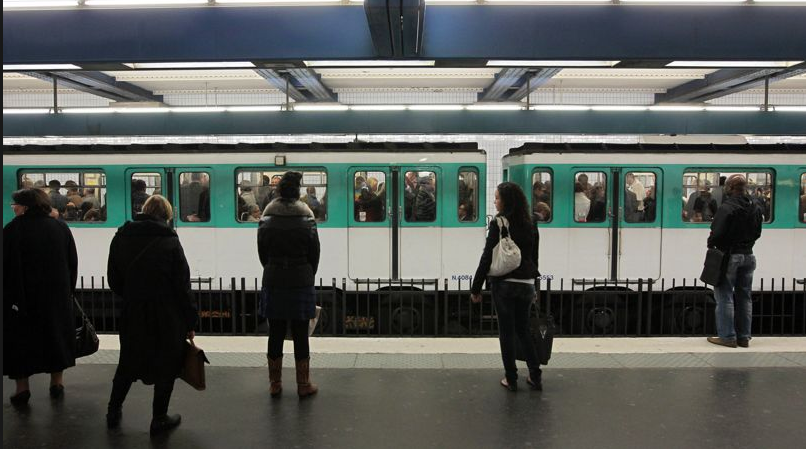
\includegraphics[width=4cm]{ratp.png}
		\caption{Some metro station}
		\label{figure}
		\end{figure}
	\end{itemize}
\end{itemize}
\end{frame}

\begin{frame}
\frametitle{Random variables}
\begin{itemize}
	\item A \textbf{random variable} is a quantity that can take several values
	\item	For instance : 
	\begin{itemize}
		\item the result of a dice throw
		\item	waiting time with RATP
		\item	weather
		\begin{figure}[!h]
		\centering
		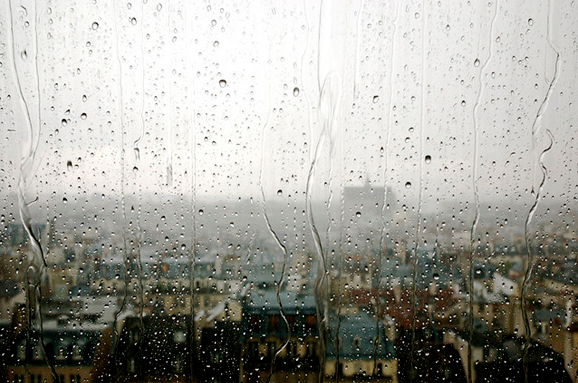
\includegraphics[width=4cm]{weather.png}
		\caption{Weather in November}
		\label{figure}
		\end{figure}
	\end{itemize}
\end{itemize}
\end{frame}


\begin{frame}
\frametitle{Random variables}
\begin{itemize}
	\item A \textbf{random variable} is a quantity that can take several values
	\item	For instance : 
	\begin{itemize}
		\item the result of a dice throw
		\item waiting time with RATP
		\item weather
		\item number of cars taking the periphérique at the same time	
	\end{itemize}
\end{itemize}
\end{frame}

\begin{frame}{Why are random variables important ?}

    \begin{itemize}
    	\item most datasets encountered in machine learning can be considered as sampled from random variables.
	\item this is important for theoretical studies, and hence for applications: a better theoretical understanding of a problem allows to choose the best algorithm to solve it.
	\item theoretical results are sometimes precise in the sense that they allow to estimate the order of magnitude of the statistical error (e.g. the prediction error) as a function of $d$ (dimension of the samples) and $n$ (number of samples)
	\item a subdomain of machine learning is "statistical learning"
    \end{itemize}

\end{frame}

\begin{frame}
\frametitle{Random variables}
\begin{itemize}
	\item Some are random variables \textbf{continuous}, others \textbf{discrete}
	\item	\textbf{continuous : }weather, RATP
	\item	\textbf{discrete : }dice (6 possibilities), number of cars ($>10000$)
\end{itemize}
\end{frame}

\begin{frame}
\frametitle{Probability distributions}

\begin{itemize}
	\item A random variable is linked to a \textbf{probability distribution}, which is a function $P$
	\item It quantifies the probability of observing one outcome.
	\item	For a discrete variable : each possible outcome is associated with a number between $0$ and $1$
\end{itemize}
\end{frame}

\begin{frame}
\frametitle{Probability distributions}
\begin{itemize}
	\item	For a dice game, the possible outcomes are  in the set $\{1,2,3,4,5,6\}$
	\item For a dice game : $P(1)= $? $P(2)= $? $P(3)= $? $P(4)= $? $P(5)= $? $P(6)= $?
\end{itemize}
\end{frame}

\begin{frame}
\frametitle{Probability distributions}
\begin{itemize}
	\item	For a dice game, the possible outcomes are  in the set $\{1,2,3,4,5,6\}$
	\item For a dice game : $P(1)=\frac{1}{6}$, $P(2)=\frac{1}{6}$, $P(3)=\frac{1}{6}$, $P(4)=\frac{1}{6}$, $P(5)=\frac{1}{6}$, $P(6)=\frac{1}{6}$
	\item	This is called a \textbf{uniform distribution}
\end{itemize}
\end{frame}


\begin{frame}
\frametitle{Probability distributions}
\begin{itemize}
	\item Periphérique : probably a time-dependent very complicated distribution 
\end{itemize}
\end{frame}

\begin{frame}
\frametitle{Continuous variables}
\begin{itemize}
	\item The situation is different for continuous random variables. 
	\item The distribution is given by a \textbf{probability density function}. Informally, the probably of being between $x$ and $x+dx$ is $p(x)dx$.
	\item \url{https://en.wikipedia.org/wiki/Probability_density_function} 
	\item Not that some variables are neither discrete nor continuous.
\end{itemize}
\end{frame}

\begin{frame}
\frametitle{Uniform discrete}
\begin{figure}[!h]
\centering
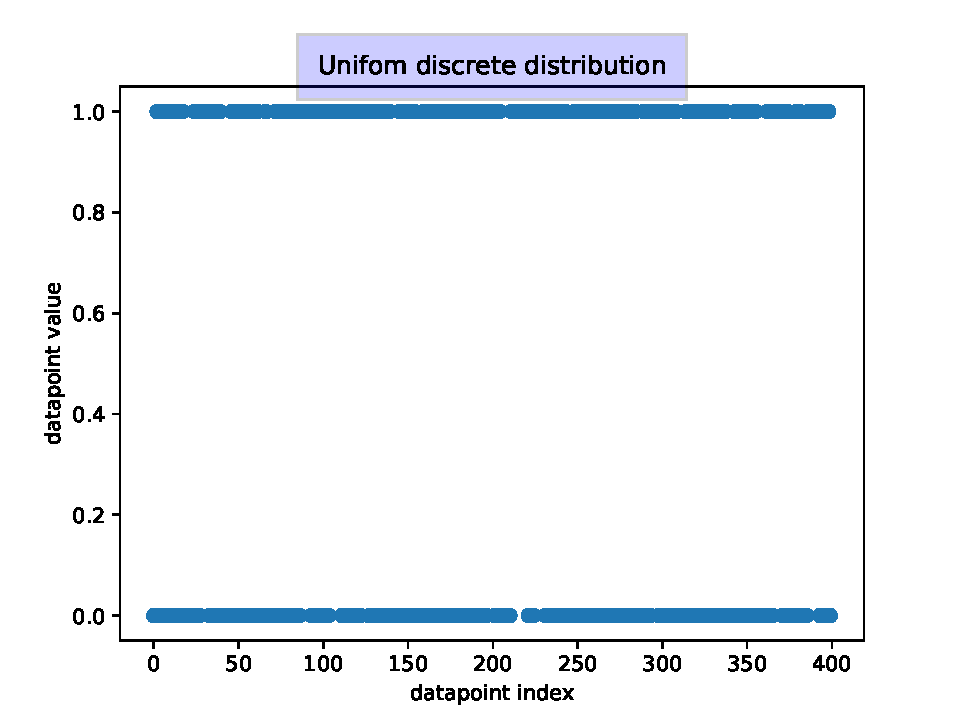
\includegraphics[width=8.5cm]{distributions/uniform_discrete_2.pdf}
\caption{Uniform discrete distribution with 2 values}
\label{figure}
\end{figure}
\end{frame}

\begin{frame}
\frametitle{Uniform discrete}
\begin{figure}[!h]
\centering
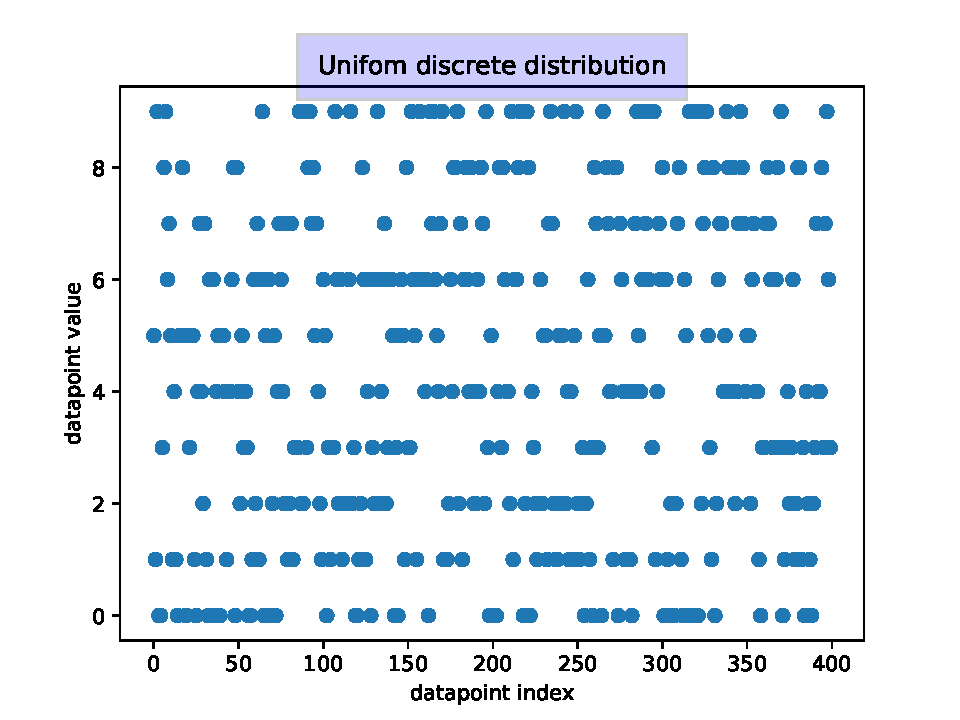
\includegraphics[width=8.5cm]{distributions/uniform_discrete_10.pdf}
\caption{Uniform discrete distribution with 10 values}
\label{figure}
\end{figure}
\end{frame}

\begin{frame}
\frametitle{Bernoulli}
\begin{figure}[!h]
\centering
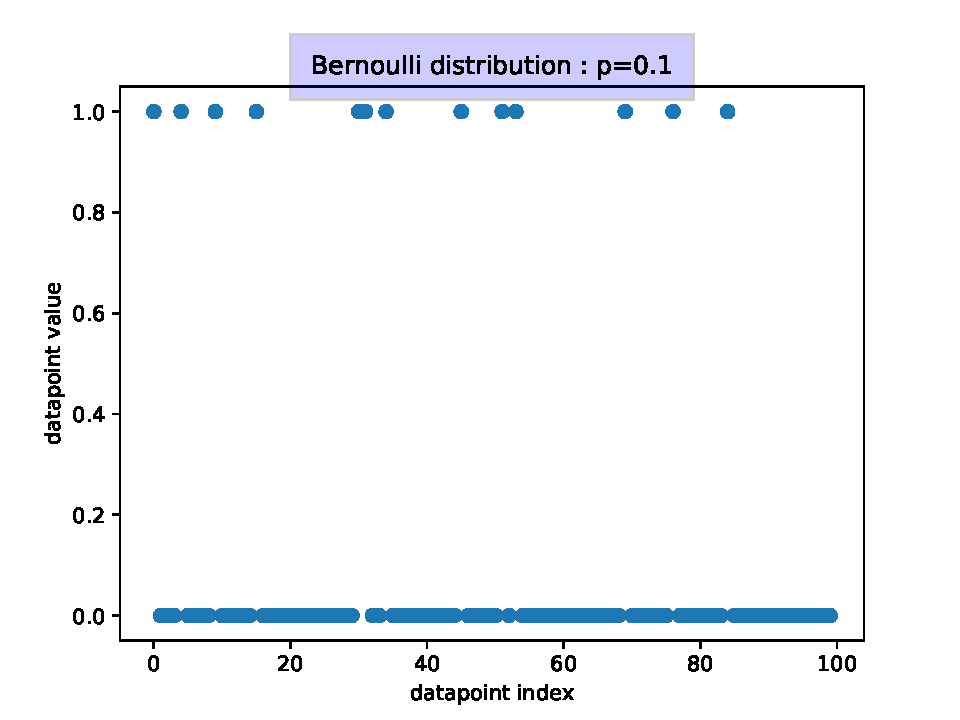
\includegraphics[width=8.5cm]{bernoulli_01.pdf}
\caption{Bernoulli distribution}
\label{figure}
\end{figure}
\end{frame}

\begin{frame}{Bernoulli p}
   \begin{itemize}
       \item With probability $p$, $X=1$
    \item With probability $1-p$, $X=0$ 
   \end{itemize} 
\end{frame}

\begin{frame}
\frametitle{Bernoulli}
\begin{figure}[!h]
\centering
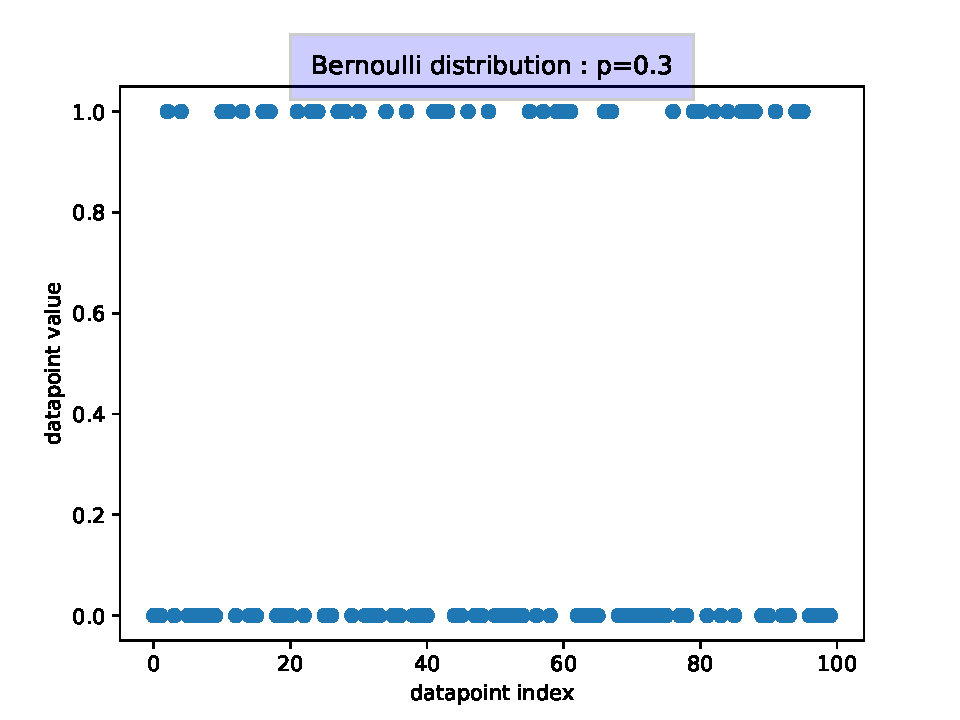
\includegraphics[width=8.5cm]{bernoulli_03.pdf}
\caption{Bernoulli Distribution}
\label{figure}
\end{figure}
\end{frame}

\begin{frame}
\frametitle{Bernoulli}
\begin{figure}[!h]
\centering
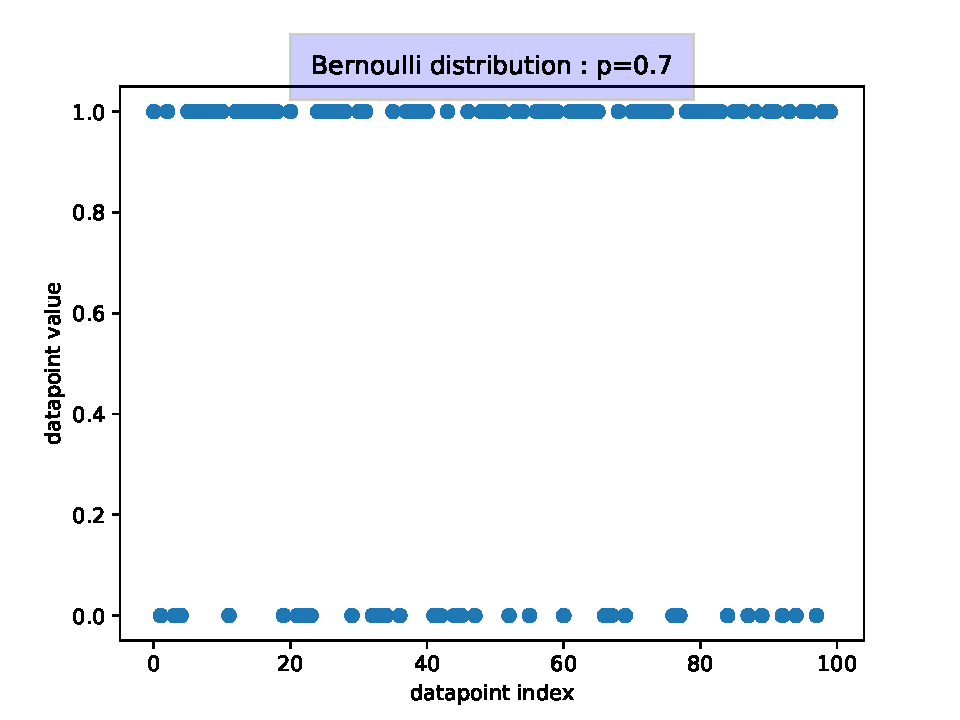
\includegraphics[width=8.5cm]{bernoulli_07.pdf}
\caption{Bernoulli Distribution}
\label{figure}
\end{figure}
\end{frame}

\begin{frame}
\frametitle{Uniform continuous}
\begin{figure}[!h]
\centering
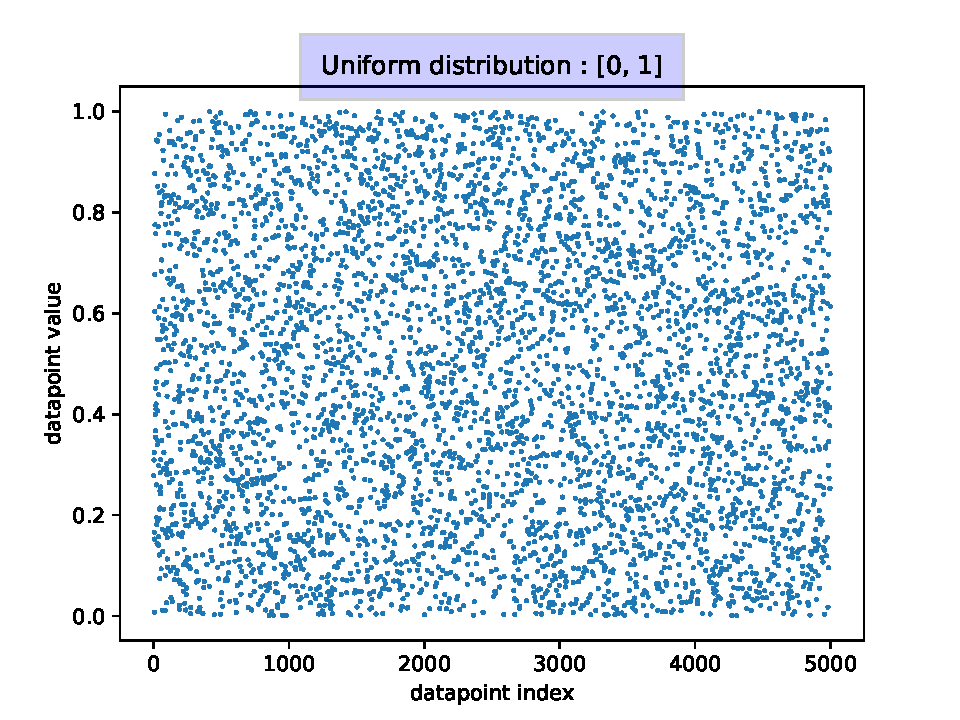
\includegraphics[width=8.5cm]{distributions/unif_continuous_01.pdf}
\caption{Uniform continuous distribution}
\label{figure}
\end{figure}
\end{frame}

\begin{frame}
\frametitle{Uniform continuous}
\begin{figure}[!h]
\centering

\includegraphics[width=8.5cm]{distributions/unif_continuous_3455.pdf}
\caption{Uniform continuous distribution}
\label{figure}
\end{figure}
\end{frame}

\begin{frame}
\frametitle{Uniform continuous}
\begin{figure}[!h]
\centering
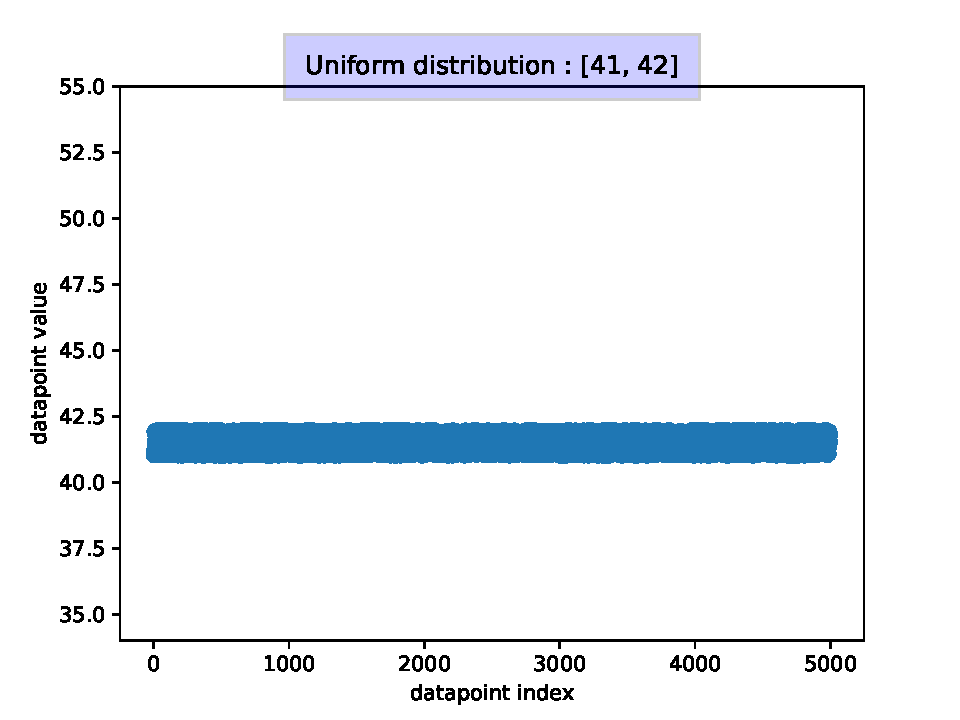
\includegraphics[width=8.5cm]{distributions/unif_continuous_41_42.pdf}
\caption{Uniform continuous distribution}
\label{figure}
\end{figure}
\end{frame}

\begin{frame}
\frametitle{Normal}
\begin{figure}[!h]
\centering
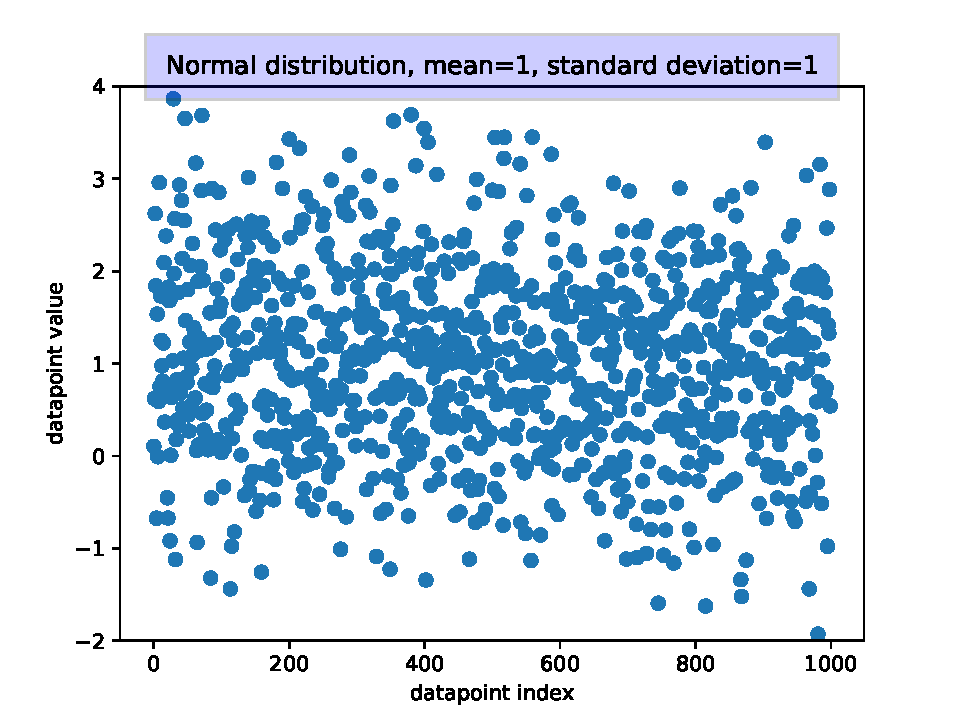
\includegraphics[width=8.5cm]{distributions/normal_m_1_std_1.pdf}
\caption{Normal distribution}
\label{figure}
\end{figure}
\end{frame}

\begin{frame}
\frametitle{Normal}
\begin{figure}[!h]
\centering
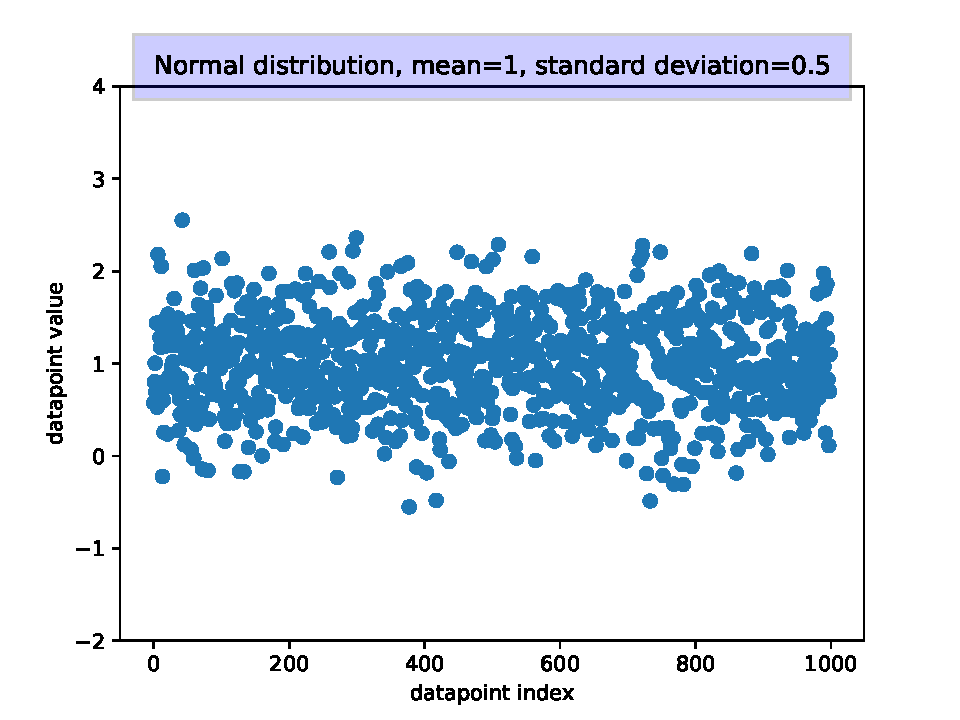
\includegraphics[width=8.5cm]{distributions/normal_m_1_std_05.pdf}
\caption{Normal distribution}
\label{figure}
\end{figure}
\end{frame}

\begin{frame}
\frametitle{Normal}
\begin{figure}[!h]
\centering
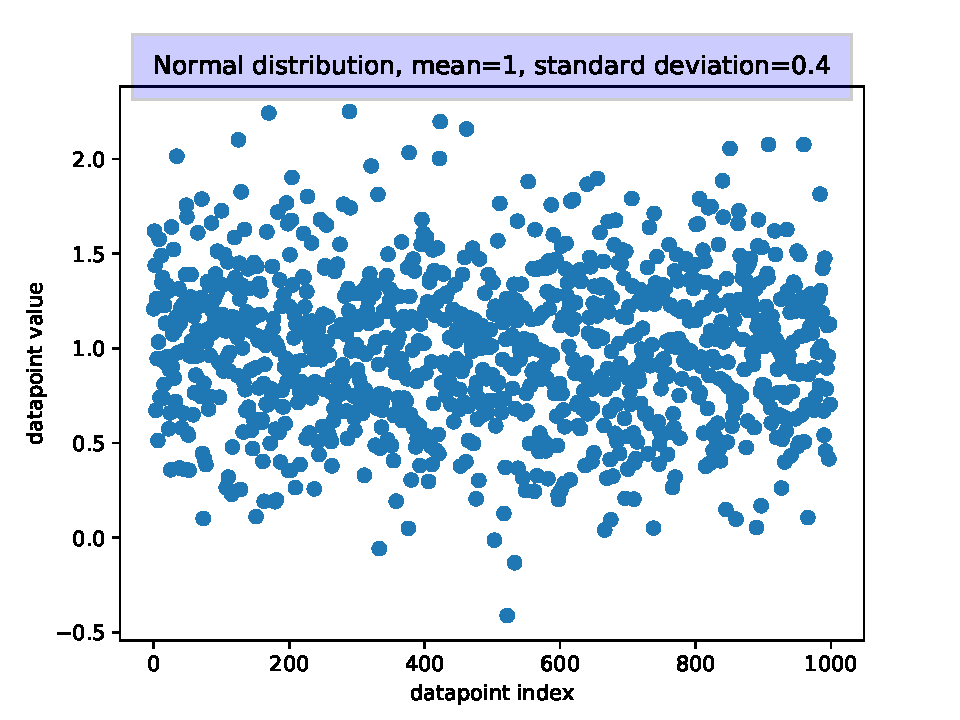
\includegraphics[width=8.5cm]{distributions/normal_m_1_std_04.pdf}
\caption{Normal distribution}
\label{figure}
\end{figure}
\end{frame}

\begin{frame}
\frametitle{White noise}
\begin{figure}[!h]
\centering
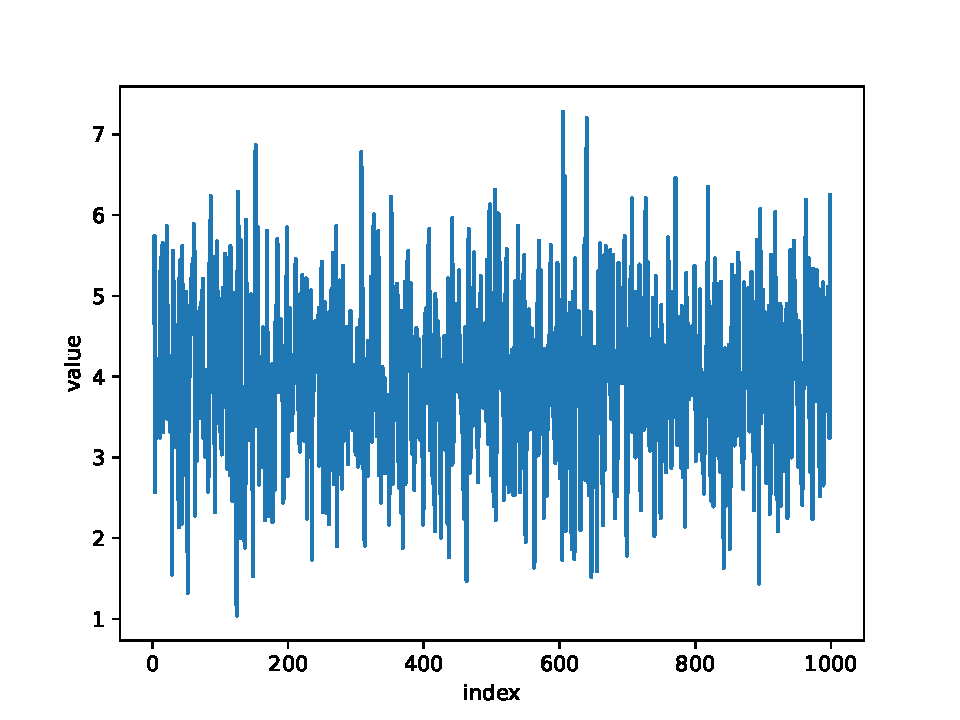
\includegraphics[width=8cm]{white.pdf}
\caption{White noise}
\label{figure}
\end{figure}
\end{frame}


\begin{frame}
\frametitle{Histograms}
    \textbf{Histograms} are an alternative representation of the results of a (one-dimensional) random variable.
\end{frame}


\begin{frame}
\frametitle{Uniform discrete}
\begin{figure}[!h]
\centering
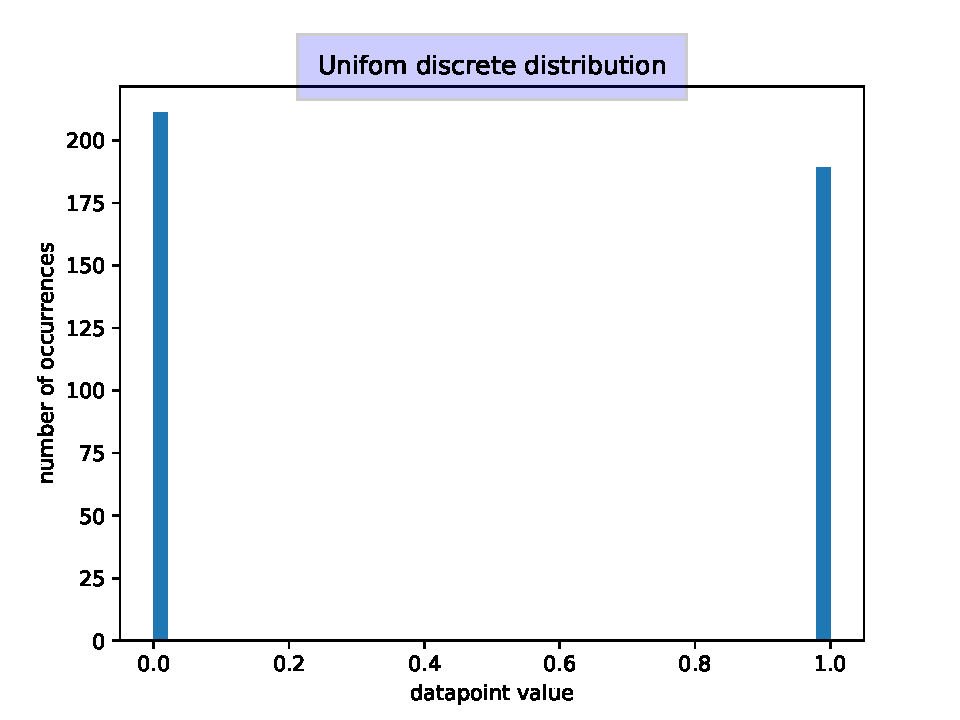
\includegraphics[width=8.5cm]{distributions/hist_uniform_discrete_2.pdf}
\caption{Historgram 1}
\label{figure}
\end{figure}
\end{frame}

\begin{frame}
\frametitle{Uniform discrete}
\begin{figure}[!h]
\centering
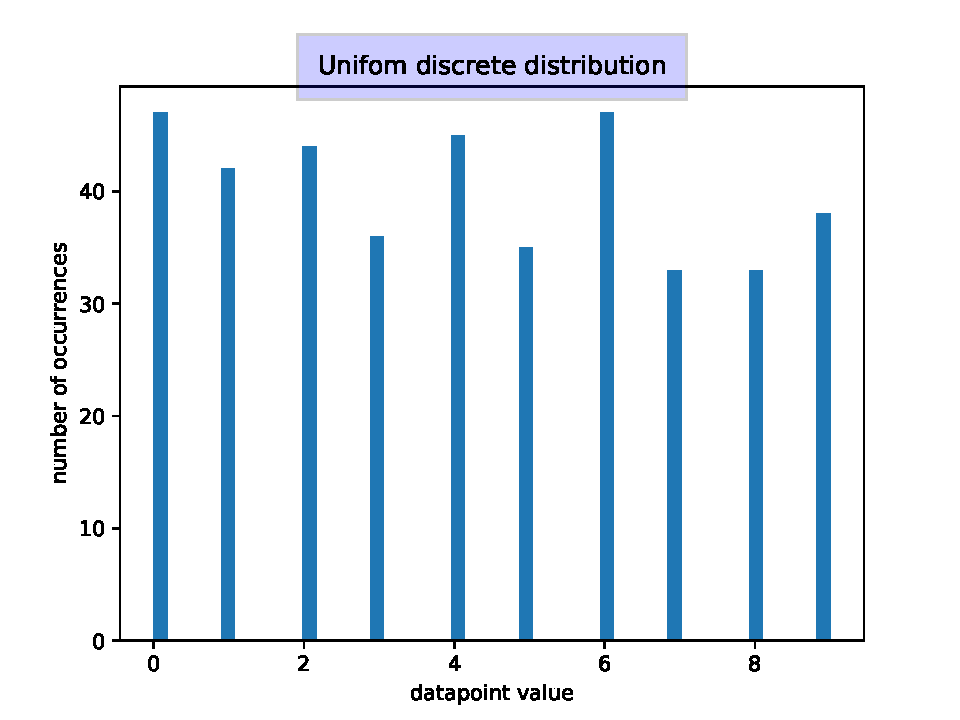
\includegraphics[width=8.5cm]{distributions/hist_uniform_discrete_10.pdf}
\caption{Historgram 1}
\label{figure}
\end{figure}
\end{frame}

\begin{frame}
\frametitle{Bernoulli}
\begin{figure}[!h]
\centering
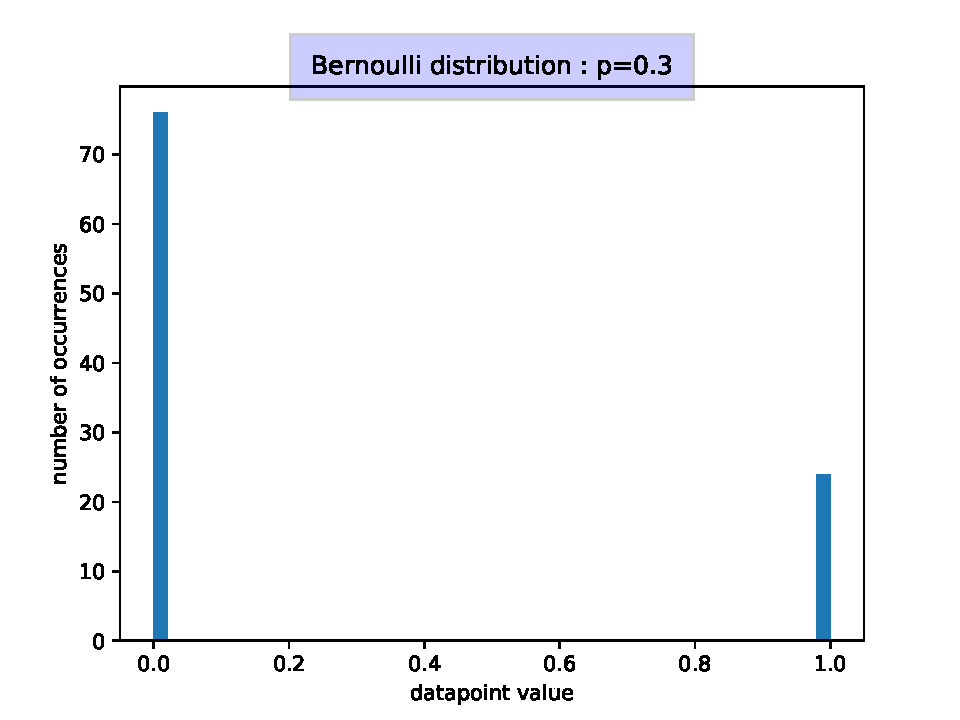
\includegraphics[width=8.5cm]{distributions/hist_bernoulli_03.pdf}
\caption{Historgram 2}
\label{figure}
\end{figure}
\end{frame}


\begin{frame}
\frametitle{Uniform continuous}
\begin{figure}[!h]
\centering
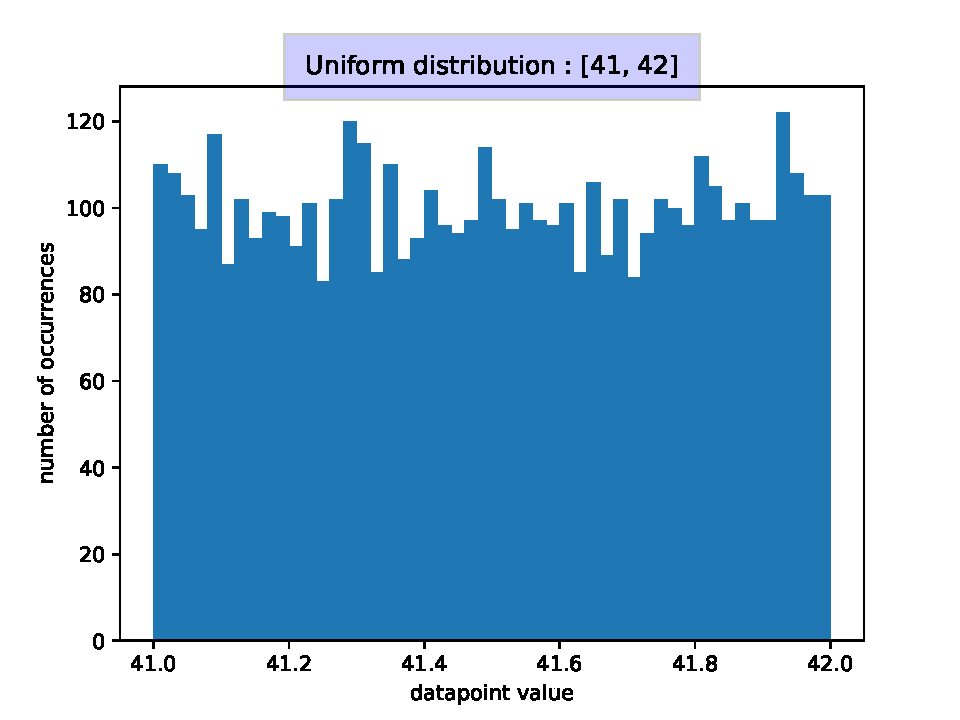
\includegraphics[width=8.5cm]{distributions/hist_unif_continuous_41_42.pdf}
\caption{Historgram 3}
\label{figure}
\end{figure}
\end{frame}

\begin{frame}
\frametitle{Normal}
\begin{figure}[!h]
\centering
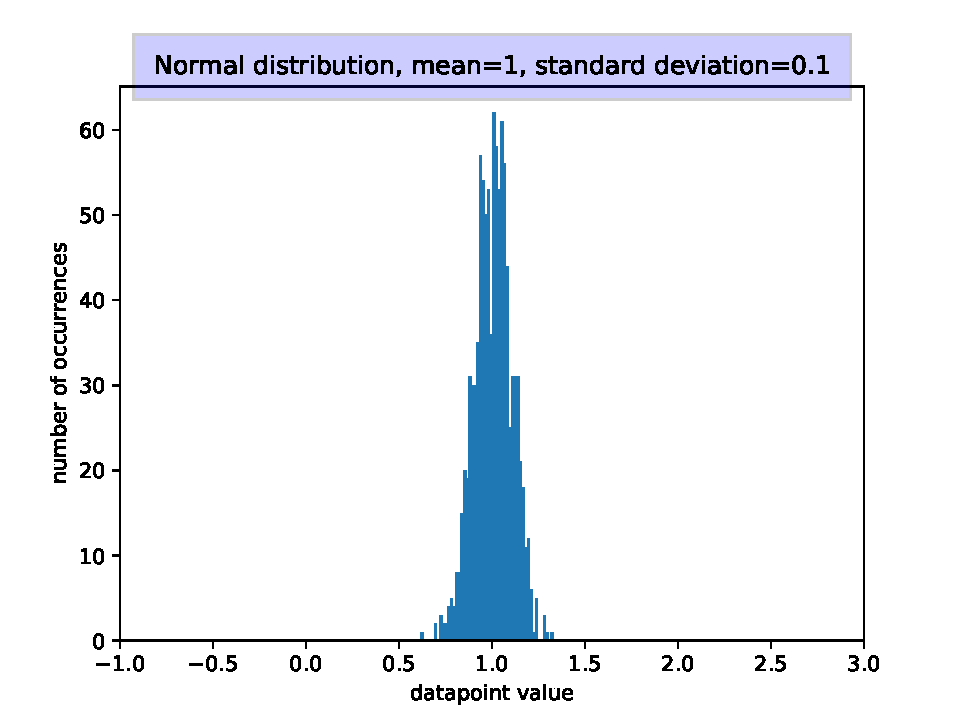
\includegraphics[width=8.5cm]{distributions/hist_normal_m_1_std_01.pdf}
\caption{Historgram 4}
\label{figure}
\end{figure}
\end{frame}

\begin{frame}
\frametitle{Normal}
\begin{figure}[!h]
\centering
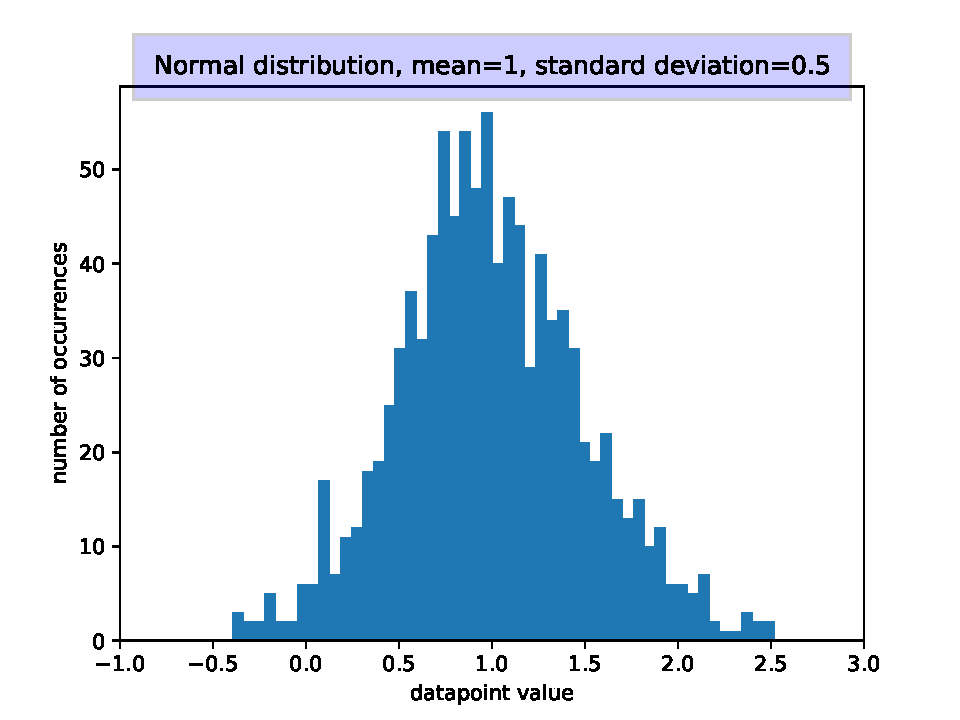
\includegraphics[width=8.5cm]{distributions/hist_normal_m_1_std_05.pdf}
\caption{Historgram 4}
\label{figure}
\end{figure}
\end{frame}

%----------------------------------------

\begin{frame}

    \textbf{cd distributions/}

    We can use the files \textbf{analyze\textunderscore distribution\textunderscore 1.py} and 
\textbf{analyze\textunderscore distribution\textunderscore 2.py} to analyze and plot some simple datasets, stored in \textbf{csv\textunderscore files/}
\end{frame}

\begin{frame}
\frametitle{Distribution 1}
\begin{figure}[!h]
\centering
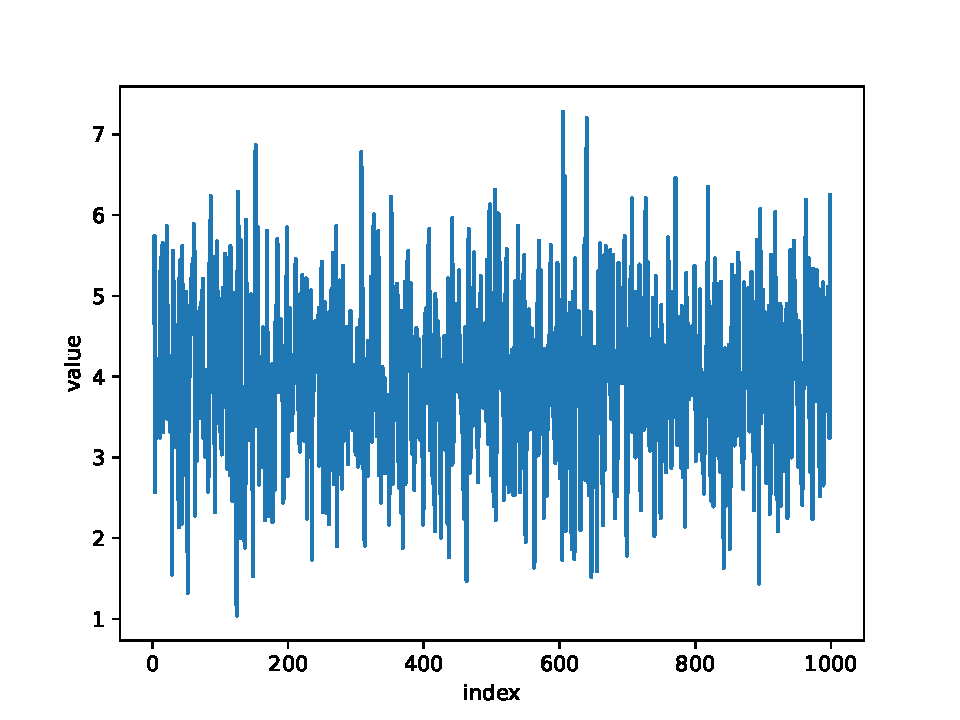
\includegraphics[width=8.5cm]{distro_1.pdf}
\caption{The data we analyze}
\label{figure}
\end{figure}
\end{frame}

\begin{frame}
\frametitle{histograms}
\begin{figure}[!h]
\centering
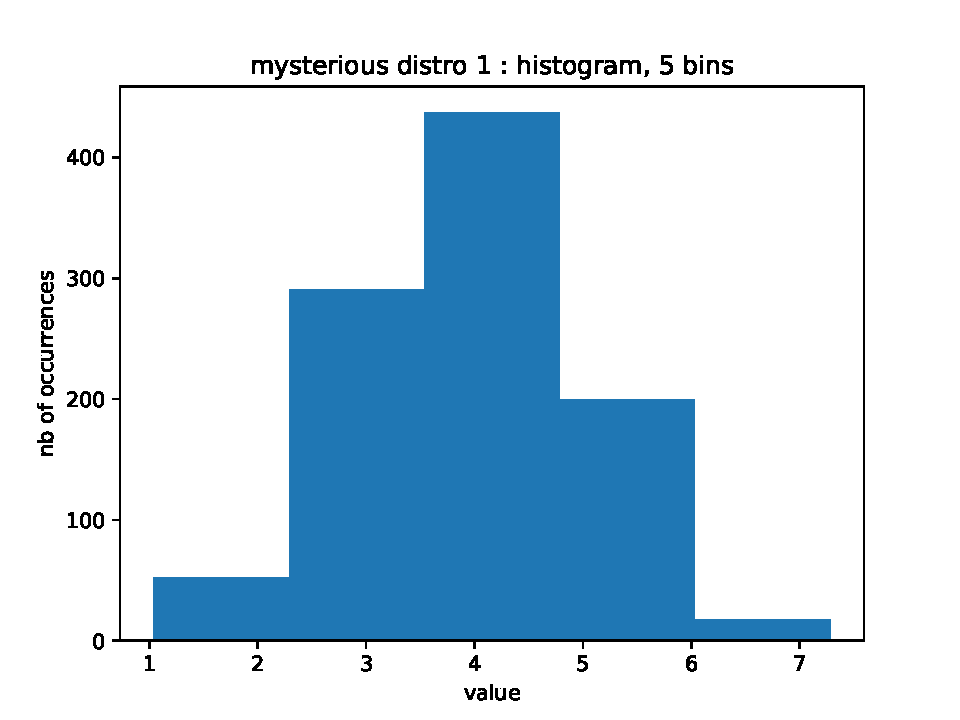
\includegraphics[width=8.5cm]{distro_1_hist_5_bins.pdf}
\caption{5 bins}
\label{figure}
\end{figure}
\end{frame}

\begin{frame}
\frametitle{histograms}
\begin{figure}[!h]
\centering
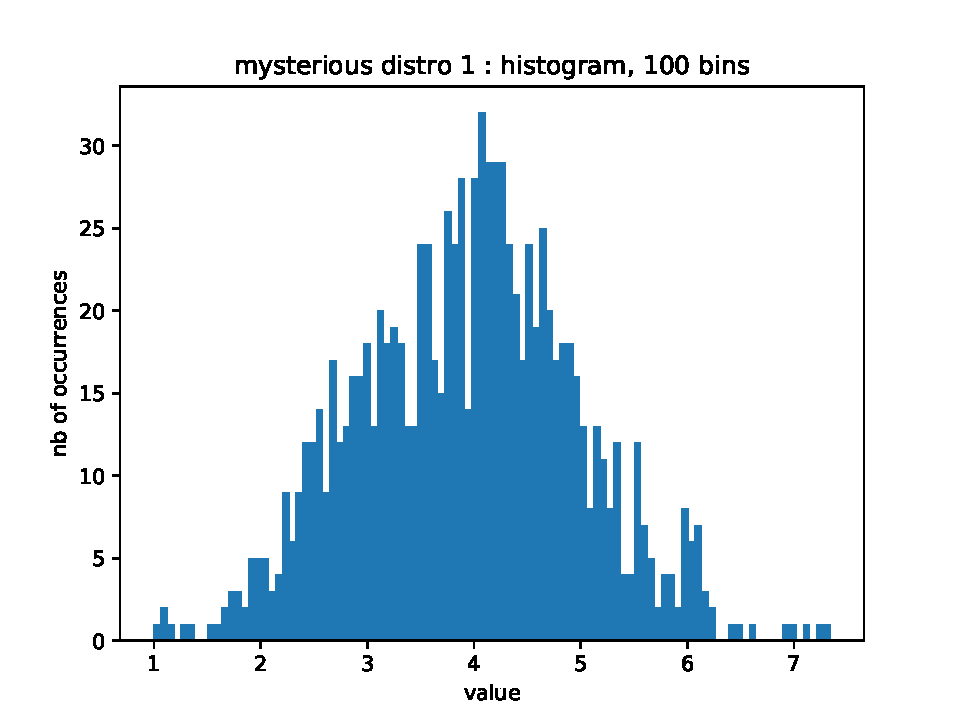
\includegraphics[width=8.5cm]{distro_1_hist_100_bins.pdf}
\caption{100 bins}
\label{figure}
\end{figure}
\end{frame}

\begin{frame}
\frametitle{histograms}
\begin{figure}[!h]
\centering
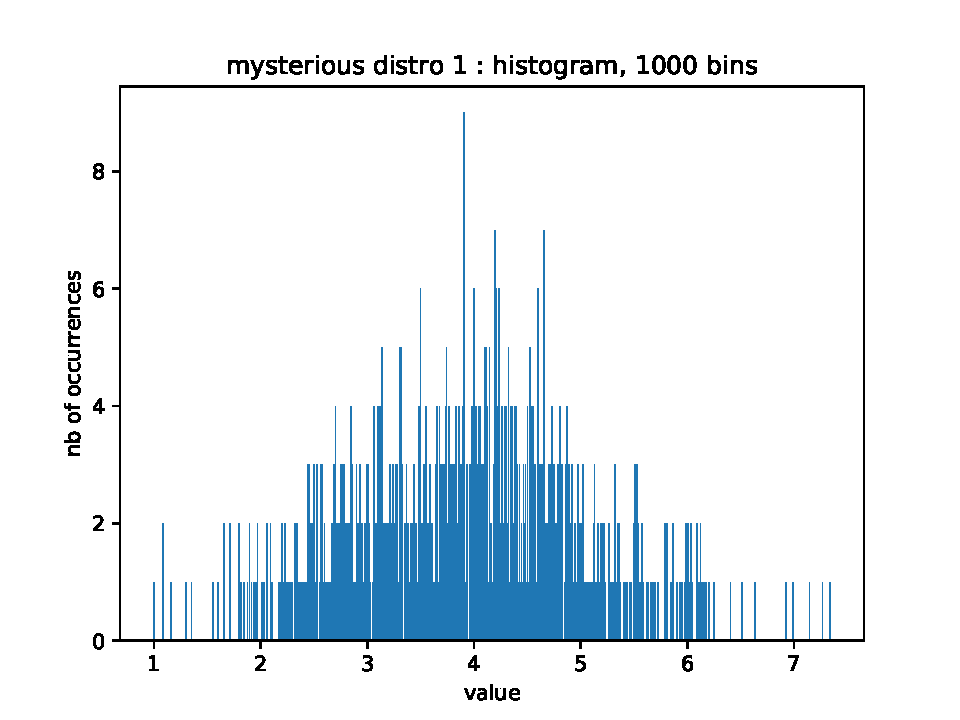
\includegraphics[width=8.5cm]{distro_1_hist_1000_bins.pdf}
\caption{1000 bins (too many)}
\label{Creation of the distribution}
\end{figure}
\end{frame}

\begin{frame}
\frametitle{Normal distribution}
\begin{figure}[!h]
\centering
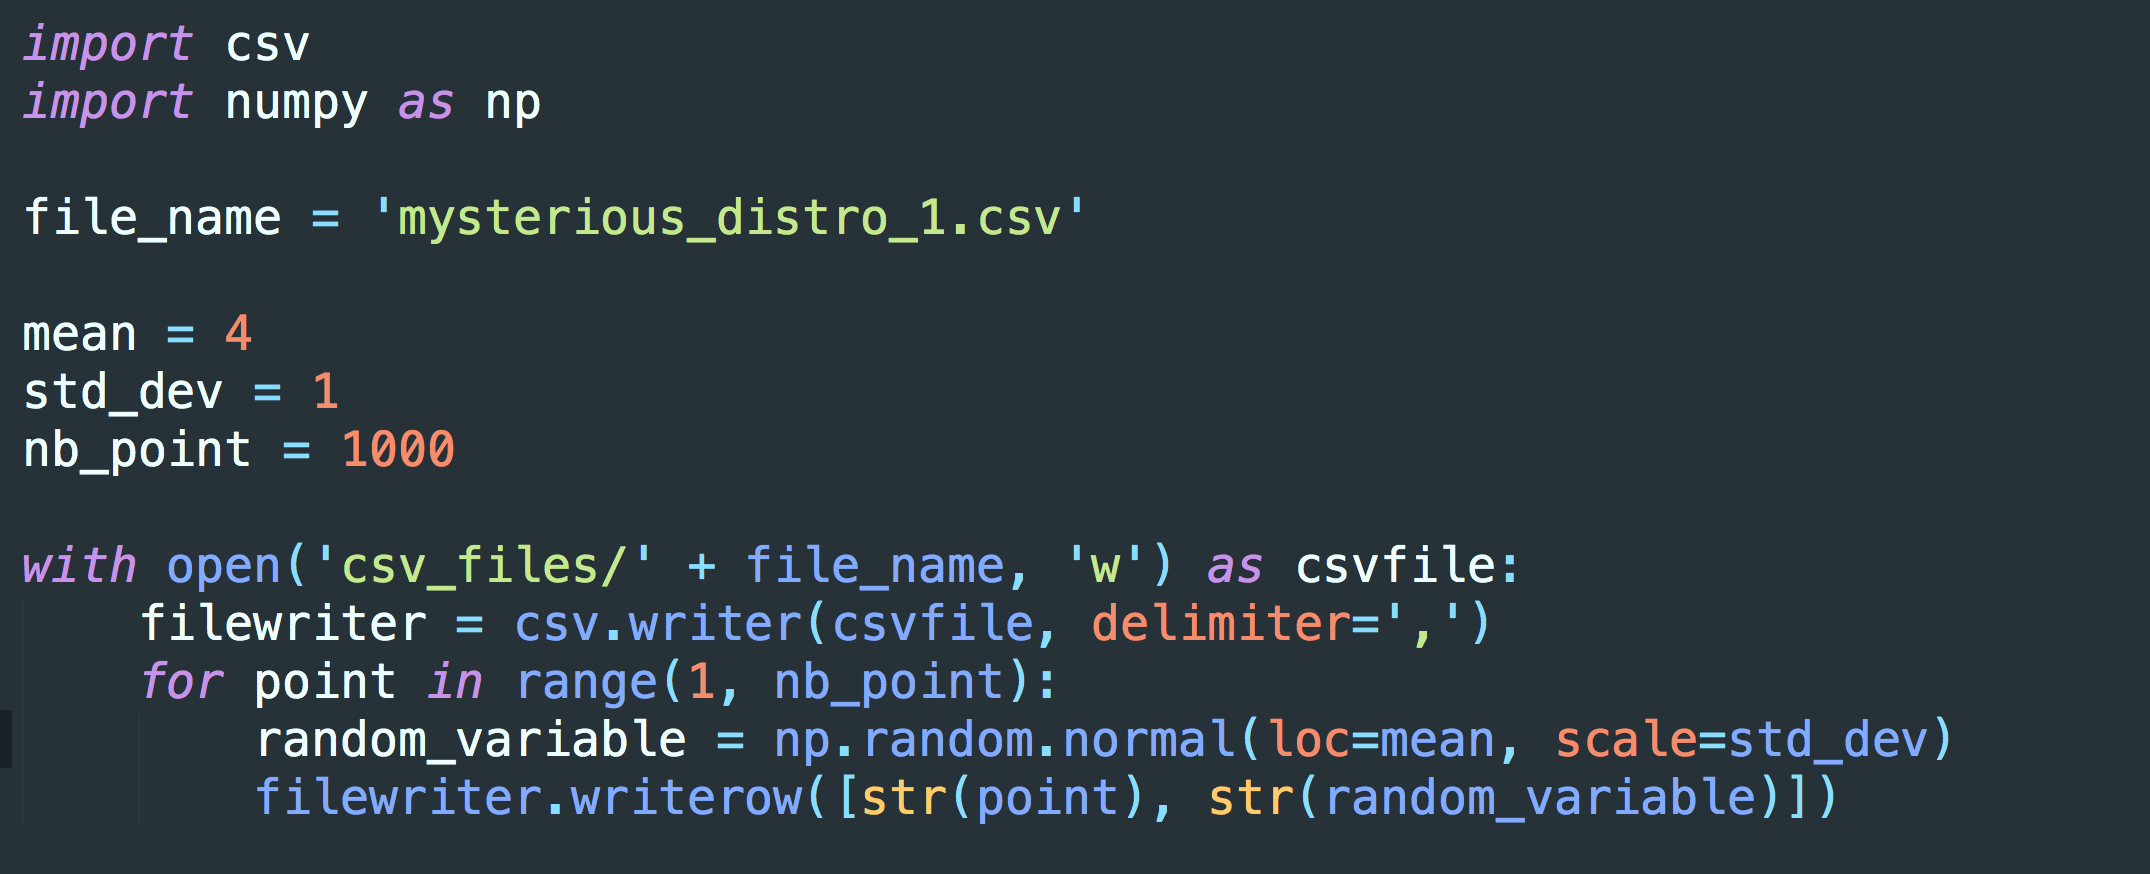
\includegraphics[width=8.5cm]{normal-creation.png}
\caption{\textbf{create\textunderscore normal.py} : Creation of the distribution}
\label{figure}
\end{figure}
\end{frame}


\begin{frame}
\frametitle{Second example}
\begin{figure}[!h]
\centering
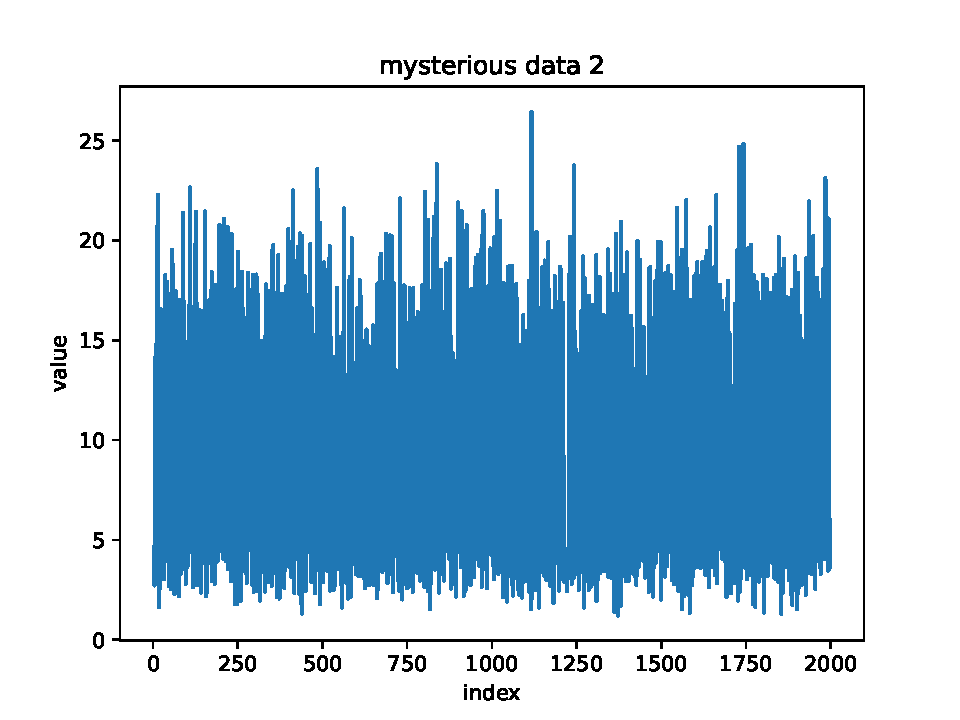
\includegraphics[width=8.5cm]{distro_2.pdf}
\caption{Second distribution}
\label{figure}
\end{figure}
\end{frame}

\begin{frame}
    \exercice{} Create a one-dimensional dataset with a histogram that looks like this one !
\begin{figure}[!h]
\centering
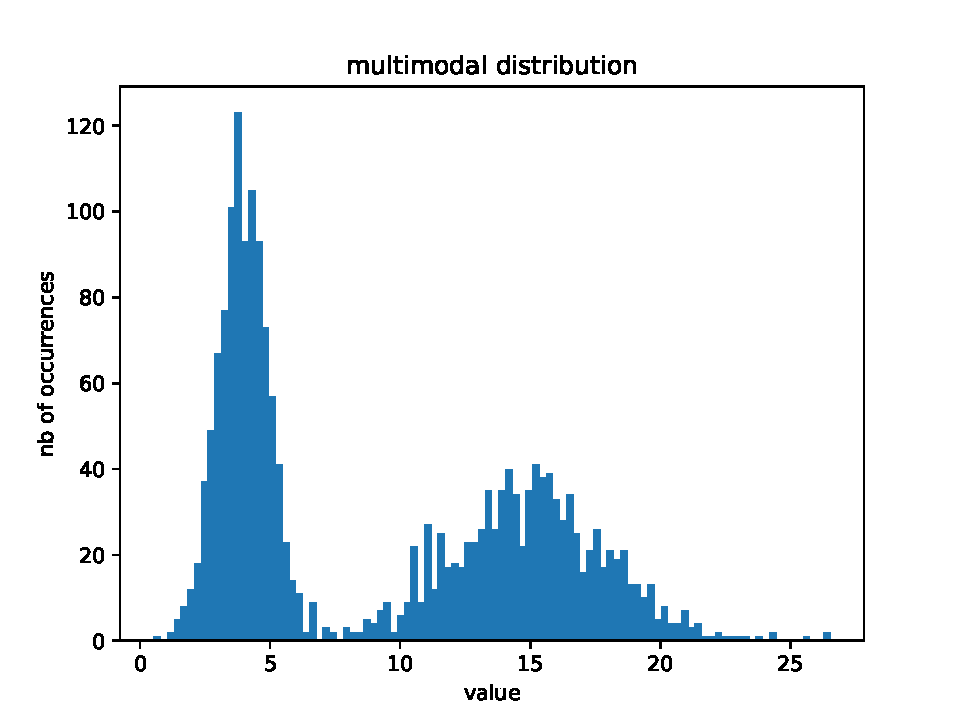
\includegraphics[width=7.2cm]{multimodal_distribution_100_bins.pdf}
\caption{This distribution has several \textbf{modes}}
\label{figure}
\end{figure}
\end{frame}

\begin{frame}{Expected value}

    \begin{itemize}
	\item The \textbf{expected value} of a random variable is its probablistic average. 
	\item Under the condition that this probabilistic average is correctly defined.
    \end{itemize}
\end{frame}

\begin{frame}{Expected value (espérance)}
   \begin{itemize}
       \item For a discrete random variable $X$ that takes the values $x_i$ with probability $p_i$: 
	   \begin{equation}
	       E(X)= \sum^{n}_{i=1} p_ix_i
	   \end{equation}
       \item For a continuous random variable $X$ with density p: 
	   \begin{equation}
	       E(X)= \int xp(x)dx
	   \end{equation}
   \end{itemize} 

    Note that $X$ may have values in $ \mathbb{R}^d$, with $d\geq 1$.
\end{frame}

\begin{frame}{Expected value (espérance) }
    \exercice{Computing an expected value}
   \begin{itemize}
       \item For a discrete random variable $X$ that takes the values $x_i$ with probability $p_i$: 
	   \begin{equation}
	       E(X)= \sum^{n}_{i=1} p_ix_i
	   \end{equation}
       \item For a continuous random variable $X$ with density: 
	   \begin{equation}
	       E(X)= \int xp(x)dx
	   \end{equation}
   \end{itemize} 
   Compute the expected value of the dice game.
\end{frame}



\begin{frame}{Variance}
    The variance is a measure of the dispersion of a random real variable.

    \url{https://en.wikipedia.org/wiki/Variance } 
   \begin{equation}
       var(X) = E\Big(\big(X-E(X)\big)^2\Big)
   \end{equation}

    Note that we can also define the variance of a multidimensonial random variable (which means a random vector). In that case, it is a matrix.
\end{frame}

\begin{frame}
\frametitle{Multidimensional vectors}
    We often consider random variables and data that live in spaces with a
    higher dimension than 2 (random vectors).
\begin{itemize}
	\item images
	\item sensor that receives \textbf{multimodal information}
\end{itemize}
\end{frame}


\begin{frame}
\frametitle{Correlation}

Random vectors with correlated components are common statistical objects.
\begin{itemize}
    \item In physics, temperature and pressure, measured by some sensores are
        correlated.
    \item In a dataset of customers of a company, some dimensions are likely to
        be correlted.
\end{itemize}

    To study the statistical relationship between components, we can compute
    the \textbf{covariance} of the two components, or the \textbf{correlation}, (normalized covariance (see below)).

    \url{https://en.wikipedia.org/wiki/Correlation} 
\end{frame}



\begin{frame}{Covariance}

    The covariance is a measure of the relationship between the variations of two random variables.
   \begin{equation}
       cov(X,Y)= E\Big( \big(X-E(X))(Y-E(Y)\big)  \Big)
   \end{equation}
\end{frame}

\begin{frame}{Correlation}
    The correlation is the covariance divided by the square roots of the variances.
   \begin{equation}
       corr(X,Y)= \frac{cov(X,Y)}{ \sqrt{Var(X)} \sqrt{Var(Y)}} 
   \end{equation}

\end{frame}

\begin{frame}
\frametitle{Example}
The data in \textbf{csv\textunderscore files/distribution\textunderscore 3.csv}
    contain samples of a random variable with $5$ dimensions (random vector). Some of these dimensions are correlated.

\end{frame}

\begin{frame}{Covariance}
   \begin{figure}[htpb]
   	\centering
   	
\includegraphics[width=0.75\textwidth]{covariance}
   	\caption{Covariance matrix of the random vector.}
   	\label{fig:covariance}
   \end{figure} 
\end{frame}

\begin{frame}
\frametitle{Correlation matrix}
\begin{figure}[!h]
\centering

\includegraphics[width=0.75\textwidth]{correlation_matrix.pdf}
\caption{Correlation matrix for the distribution, note the difference in the scale.}
\label{figure}
\end{figure}
\end{frame}

\begin{frame}{Pandas, scikit-learn}

	\begin{itemize}
		\item \url{https://pandas.pydata.org/} 
		\item \url{https://scikit-learn.org/stable/datasets/toy_dataset.html} 
		\item pandas demo with iris and distribution 3.
	\end{itemize}

\end{frame}

\section{Optimization}

\begin{frame}{Minimization of a function}

    Optimization is another core aspect of machine learning.


\begin{figure}[htpb]
    \centering
    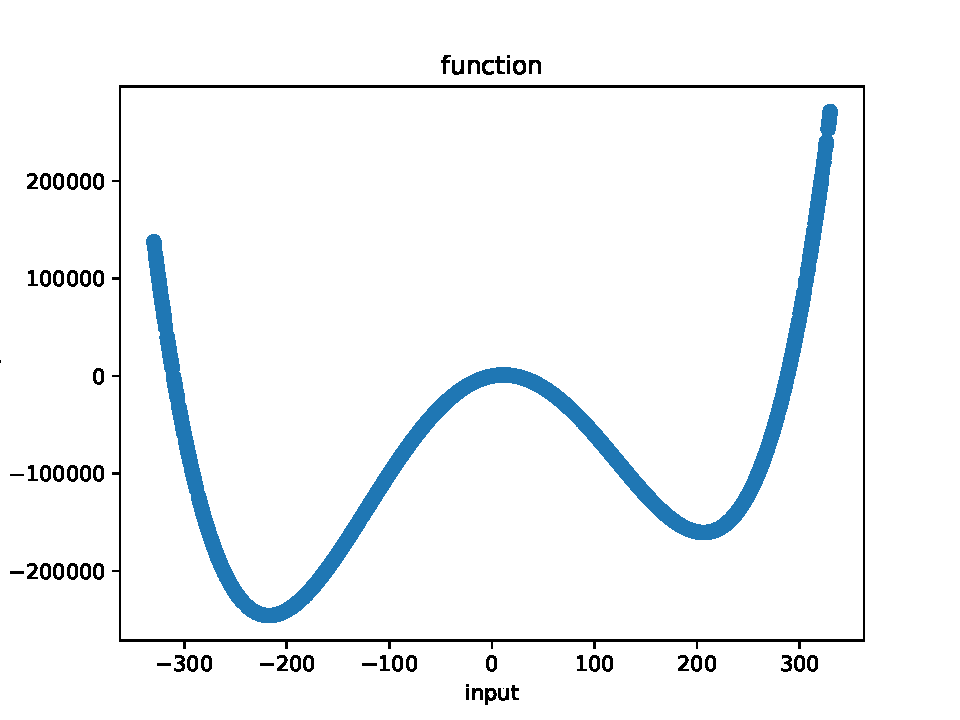
\includegraphics[width=0.7\linewidth]{function}
    \label{fig:function}
    \caption{Loss function}
\end{figure}    

\end{frame}

\begin{frame}{Optimization in machine learning}
The loss function typically represents the quality of a set of parameters to
    solve a problem.
    \begin{itemize}
        \item in supervised learning, typically a measure of the prediction
            error on the dataset
        \item in clustering, typically a distorsion
        \item in density estimation, a likelihood
    \end{itemize}

\end{frame}

\begin{frame}{Analytic minimization}
    \exercice{}
   What is the minimum of the function
    \begin{equation}
        f : x \rightarrow (x-1)^2+3.5
    \end{equation}
    And for what value $x$ is it obtained ?
\end{frame}

\begin{frame}{Iterative algorithms}

    However, in most applications of machine learning, it is not possible to
    use an analytical solution, either because:
    \begin{itemize}
        \item we do not know the analytical solution
        \item we know how to compute it, but the computation is too costly for
            practical use.
    \end{itemize}

    Instead, we use \textbf{iterative algorithms} (gradient descent, coordinate
    descent, etc.)

\end{frame}


\begin{frame}{Gradient algorithms}

    \begin{figure}[htpb]
    	\centering
    	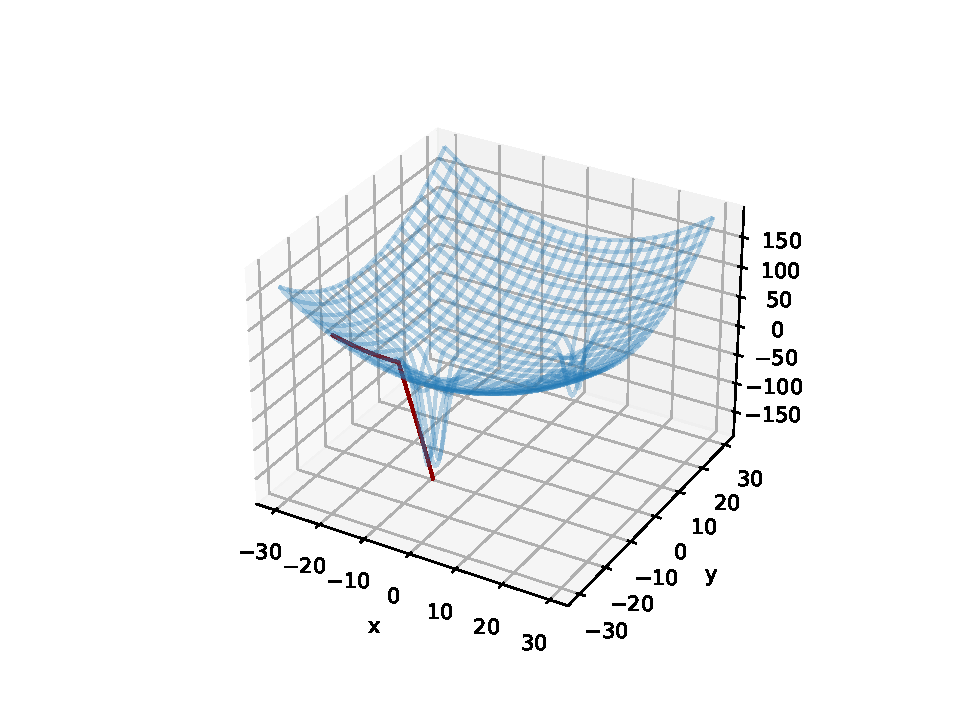
\includegraphics[width=0.75\textwidth]{8000}
    	\caption{Optimization trajectory.}
    	\label{fig:8000}
    \end{figure}
\end{frame}

\section{Metrics}%
\label{sec:Metrics}

\begin{frame}{Metrics}

    Let $D = \{x_1, \dots, x_n\}\subset \mathcal{X} $ be a dataset of $n$ samples, with labels $\{y_1, \dots, y_n\} \subset \mathcal{Y}$.

    There is a metric in the input space $ \mathcal{X}$ and in the output space $ \mathcal{Y}$.
    \begin{itemize}
    	\item The \textbf{metric} in $ \mathcal{X}$ determines to what extent two samples $x_i$ and $x_j$ should be considered similar or dissimilar.
	\item The \textbf{metric} in $ \mathcal{Y}$ determines to what extent two labels $y_i$ and $y_j$ should be considered similar or dissimilar.
    \end{itemize}

    In all machine learning, the choice of the metric is very important !
\end{frame}


\subsection{Metrics in output space}


\begin{frame}{Metrics in output space}

    A \textbf{{loss function}} $l$ is a map that measures the discrepancy between to elements of a set (for instance of a linear space).
$$
l: \left\{
    \begin{array}{ll}
	\mathcal{Y} \times \mathcal{Y} \rightarrow \mathbb{R}_+ & \\
	(y,z) \mapsto l(y,z)& 
    \end{array}
\right.
$$
    Typically, $z$ can represent our prediction for a given input $x$, $z= \tilde{f}(x)$, and $y$ the correct label.

\end{frame}

\begin{frame}{Most common supervised learning losses}

    \textbf{"0-1" loss for \textbf{{binary classification.}}}

     $ \mathcal{Y}  = \{0, 1\}$ or $ \mathcal{Y}  = \{-1, 1\}$.

	\begin{equation}
	    l(y,z) = 1_{y\neq z}
	\end{equation}

	\textbf{Squared loss for \textbf{{regression}}}

$ \mathcal{Y}  = \mathbb{R} $. 

	\begin{equation}
	    l(y,z) = (y-z)^2
	\end{equation}

\textbf{absolute loss for \textbf{{regression}}.}

$ \mathcal{Y}  = \mathbb{R} $. 

	\begin{equation}
	    l(y,z) = |y-z|
	\end{equation}
\end{frame}

\begin{frame}

    In \textbf{unsupervised learning}, there is notion of \textbf{output space !}

\end{frame}

\subsection{Metrics in input space}

\begin{frame}{Geometric distances}

    Often, $ \mathcal{X}= \mathbb{R}^p$ (input space). In this case, \textbf{geometric} metrics are used.
    $x=(x_1,...,x_p)$ and $y=(y_1,...,y_p)$ are $p$-dimensional \textbf{vectors}.
    \begin{itemize}
	\item L$2$ : $||x-y||_2=\sqrt{\sum_{k=1}^{p} (x_k-y_k)^2}$ (Euclidian distance, $2$-norm distance)
	\item L$1$ : $||x-y||_1=\sum_{k=1}^{p} |x_k-y_k|$ (Manhattan distance, $1$-norm distance)
	\item weighted $L_1$ :  $\sum_{k=1}^{p} w_k|x_k-y_k|$, with each $w_k>0$.
	\item $||x-y||_{\infty}$ : $\max ( |x_i-y_i|, i\in[1, n])$ (infinity norm distance, Chebyshev distance)
    \end{itemize}
\end{frame}


\begin{frame}{Choice of the metric}
    In some contexts, some usual metrics such as $L2$ might not be meaningful !

    \begin{figure}[htpb]
        \centering
        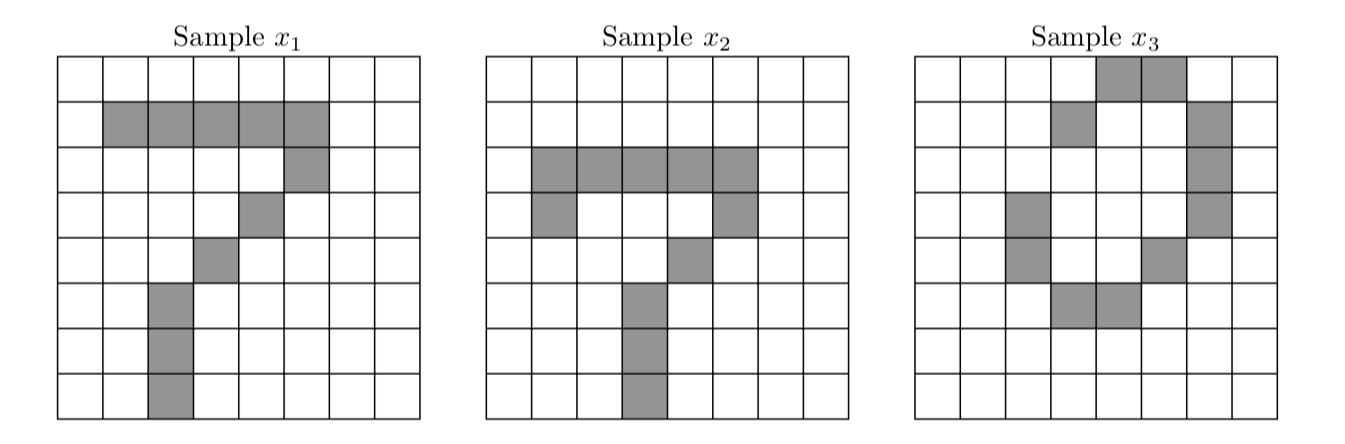
\includegraphics[width=0.8\linewidth]{supelec}
	\caption{In $ \mathbb{R}^{64}$, those three points form an equilateral triangle, \cite[]{Fix}}
        \label{fig:supelec}
    \end{figure}
\end{frame}

\begin{frame}{Non-geometric data}

    Not all data are geometric !

\end{frame}

\begin{frame}
    \frametitle{Hamming distance}
    \begin{itemize}
	\item  $\#\{x_i\neq y_i\}$ (Hamming distance)
	\item Levenshtein distance for strings (allows deletions and additions)
    \end{itemize}
\end{frame}

\begin{frame}
    \frametitle{General definition of a distance}
    A \textbf{distance}  on a set $E$ is an application $d : E\times E \rightarrow \mathbb{R}_+$ that must : 
    \begin{itemize}
	\item be \textbf{symetric} : $\forall x,y, d(x,y)=d(y,x)$
	\item \textbf{separate the values} : $\forall x,y, d(x,y)=0\Leftrightarrow x=y$
	\item	respect the \textbf{triangular inequality} $\forall x,y,z, d(x,y)\leq d(x,z)+d(y,z)$
    \end{itemize}
\end{frame}

\begin{frame}
    \frametitle{General definition of a distance}
    We could verify that : 
    \begin{itemize}
	\item L$2$ is a distance
	\item Hamming is a distance
    \end{itemize}
\end{frame}

\begin{frame}{Similarities}
    Sometimes, it is not possible to define a proper \textbf{distance} in the input space $ \mathcal{X}$ ! This may happen for instance is $ \mathcal{X}$ is a dataset of texts.
    \begin{itemize}
	\item When distances are unavailable, we can use \textbf{{Similarities}} or \textbf{{Dissimilarity}} to compare points.
	\item Dissimilarites are more general and don't always abide by the
	    distance axioms.
	\item Other examples: Adjacency in an oriented graph, Custom agregated score to compare data. 
    \end{itemize}
\end{frame}

\begin{frame}{Example: cosine similarity}

    The \textbf{{cosine similarity}} may be used to compare texts.

    If $u$ and $v$ are vectors,
    \begin{equation}
	S_C(u, v) = \frac{(u|v)}{||u|| ||v||} 
    \end{equation}

    \begin{itemize}
	\item the \textbf{{bag of words representation}} allows us to build a vector from a text (one hot encoding).
	\item \textbf{{cosine\textunderscore similarity/scraper.py}} 
	\item \textbf{{cosine\textunderscore similarity/similarity.py}} 
    \end{itemize}
\end{frame}


\begin{frame}{Hybrid data}

    Sometimes each sample contains both numerical data and non-numerical data (text, categorical data.)

    See \textbf{day\textunderscore 1/4\textunderscore metrics/hybrid\textunderscore data/}

    This is often the case in machine learning applications ! (database of customers, cars, countries, etc.)

\end{frame}

\begin{frame}
   \exercice{}Using the notebook in \textbf{day\textunderscore 1/4\textunderscore metrics/geometric\textunderscore data/},
    choose the metric and the threshold so that this graph (and the ones on the next slides) are built.

    \begin{figure}[htpb]
    	\centering
    	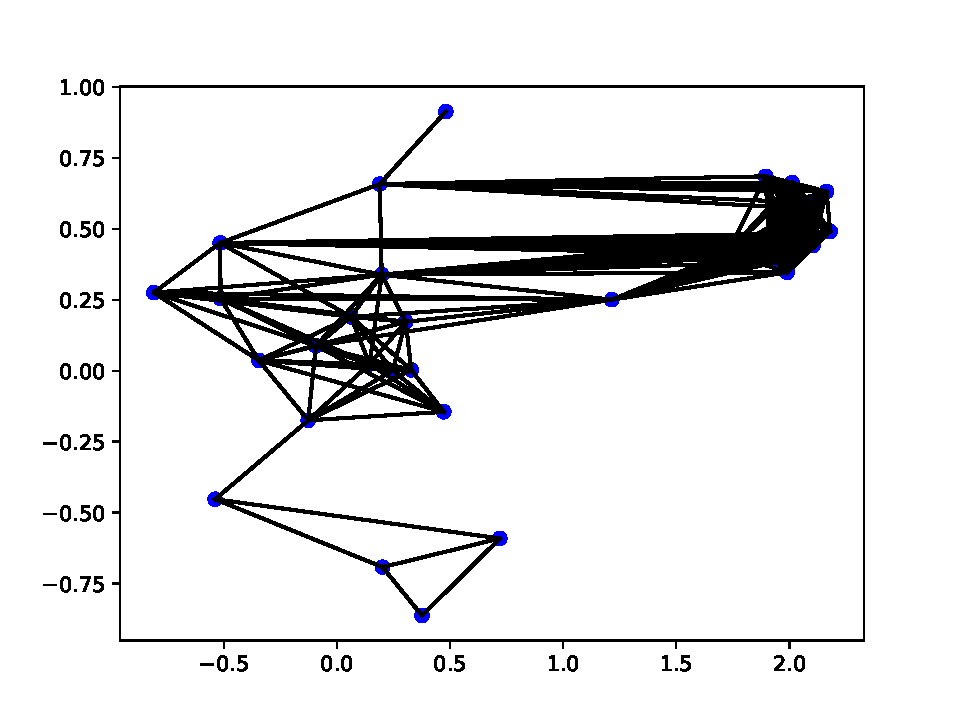
\includegraphics[width=0.6\textwidth]{thres_0_3_dist_weighted_manhattan}
    \end{figure}
\end{frame}

\begin{frame}{}
    \begin{figure}[htpb]
    	\centering
    	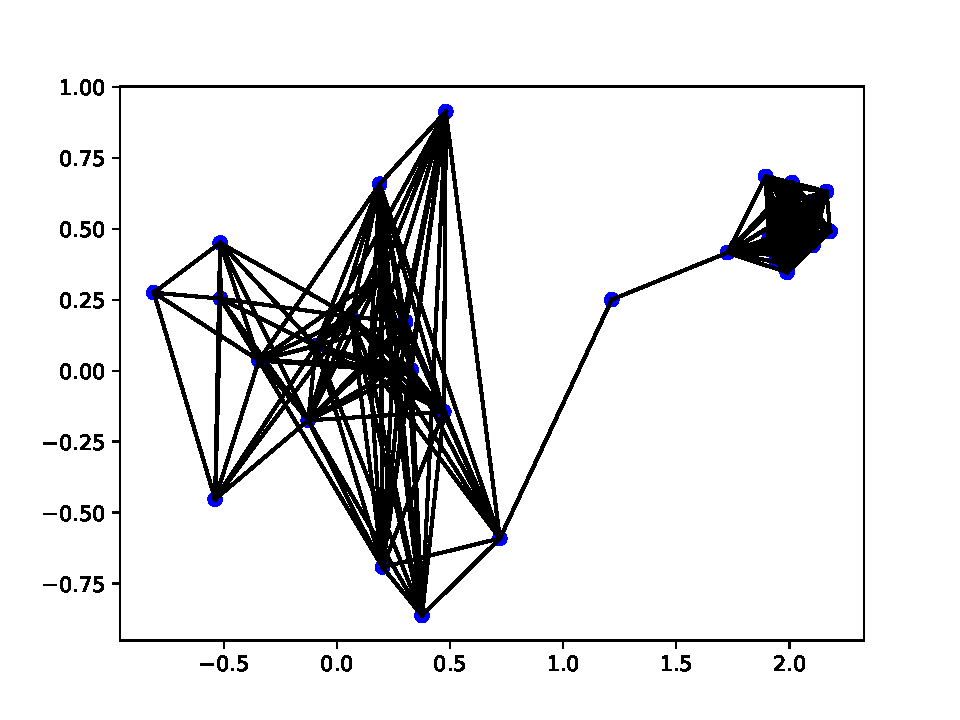
\includegraphics[width=0.8\textwidth]{thres_0_4_dist_weighted_manhattan}
    	\label{fig:thres_0_4_dist_weighted_manhattan}
    \end{figure}
\end{frame}

\begin{frame}{}
    \begin{figure}[htpb]
    	\centering
    	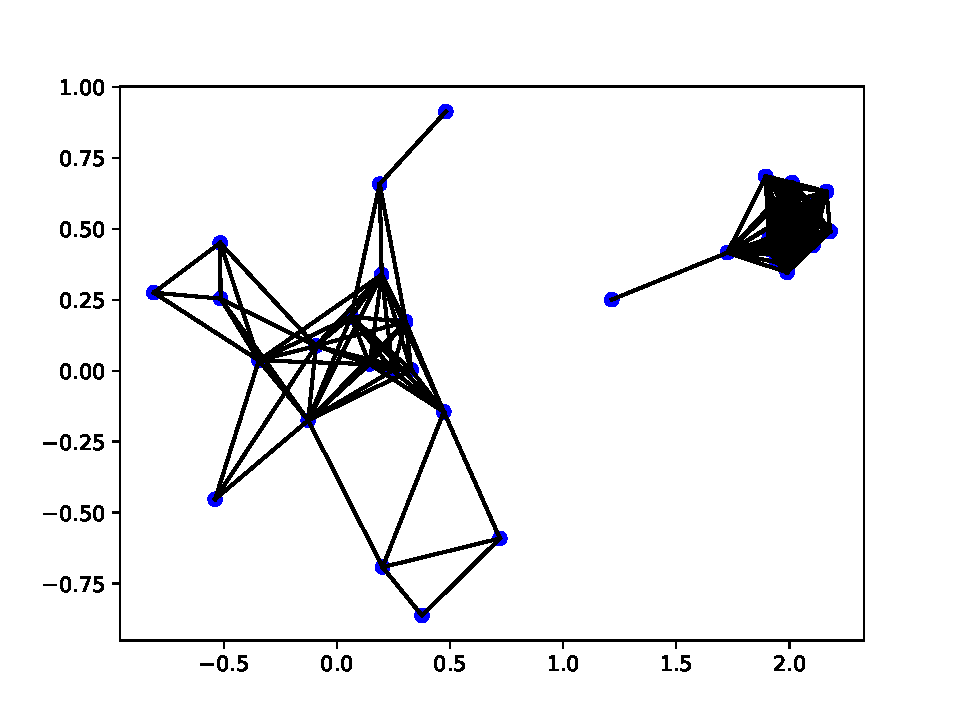
\includegraphics[width=0.8\textwidth]{thres_0_55_dist_infinie}
    	\label{fig:thres_0_55_dist_infinie}
    \end{figure}
\end{frame}

\subsection{Outliers}

\begin{frame}{Outliers}
    \textbf{Outliers} are samples that are considered like non-representative of the dataset (e.g. due to a measurement error). The detection of outliers depends on the metric !

    \begin{figure}[htpb]
    	\centering
    	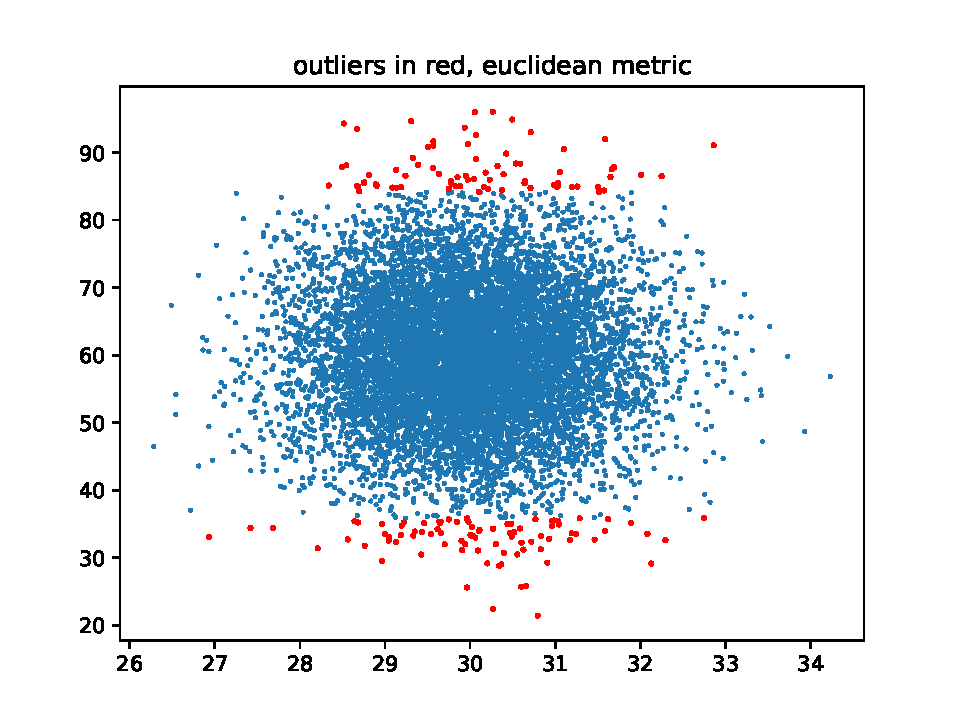
\includegraphics[width=0.6\textwidth]{outliers_metric=euclidean}
    	\caption{}
    	\label{fig:}
    \end{figure}

\end{frame}

\begin{frame}{Outliers with a different metric}

    \begin{figure}[htpb]
    	\centering
    	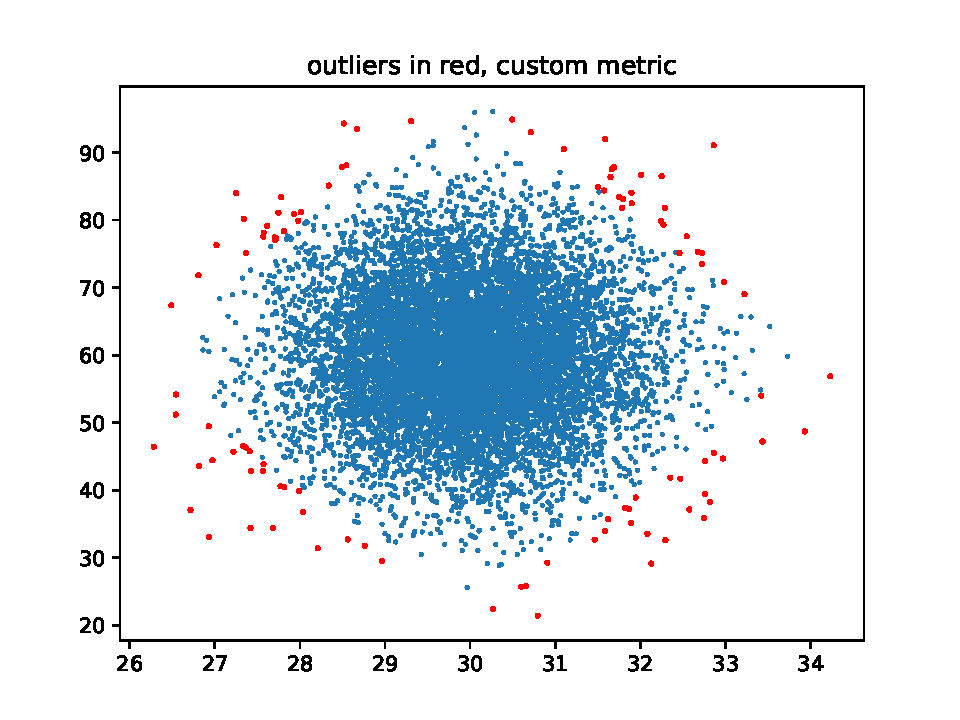
\includegraphics[width=0.8\textwidth]{outliers_metric=custom}
    	\label{fig:}
    \end{figure}

\end{frame}

\begin{frame}[allowframebreaks]
\frametitle{References}
\bibliographystyle{apalike}
\bibliography{../../../../../refs.bib} 
\end{frame}

\end{document} 
